\documentclass[12pt,a4paper]{article}
\usepackage[top=3cm,bottom=2cm,left=3cm,right=2cm]{geometry}
\usepackage{mathptmx}
\usepackage{amsmath,amssymb}
\usepackage{booktabs}
\usepackage{hyperref}
\usepackage{titlesec}
\usepackage{enumitem}
\usepackage{tikz}
\usetikzlibrary{arrows.meta,positioning,shapes.geometric,calc,fit}

\hypersetup{
    colorlinks=true,
    linkcolor=black,
    urlcolor=blue,
    citecolor=black
}

\titlespacing*{\section}{0pt}{10pt}{4pt}
\titlespacing*{\subsection}{0pt}{8pt}{3pt}
\setlength{\parindent}{0pt}
\setlength{\parskip}{5pt}
\sloppy

\begin{document}
\thispagestyle{empty}
\begin{center}\textbf{1/1}\end{center}
\vspace{6pt}
\begin{figure}[h!]
\centering
\resizebox{\textwidth}{!}{%
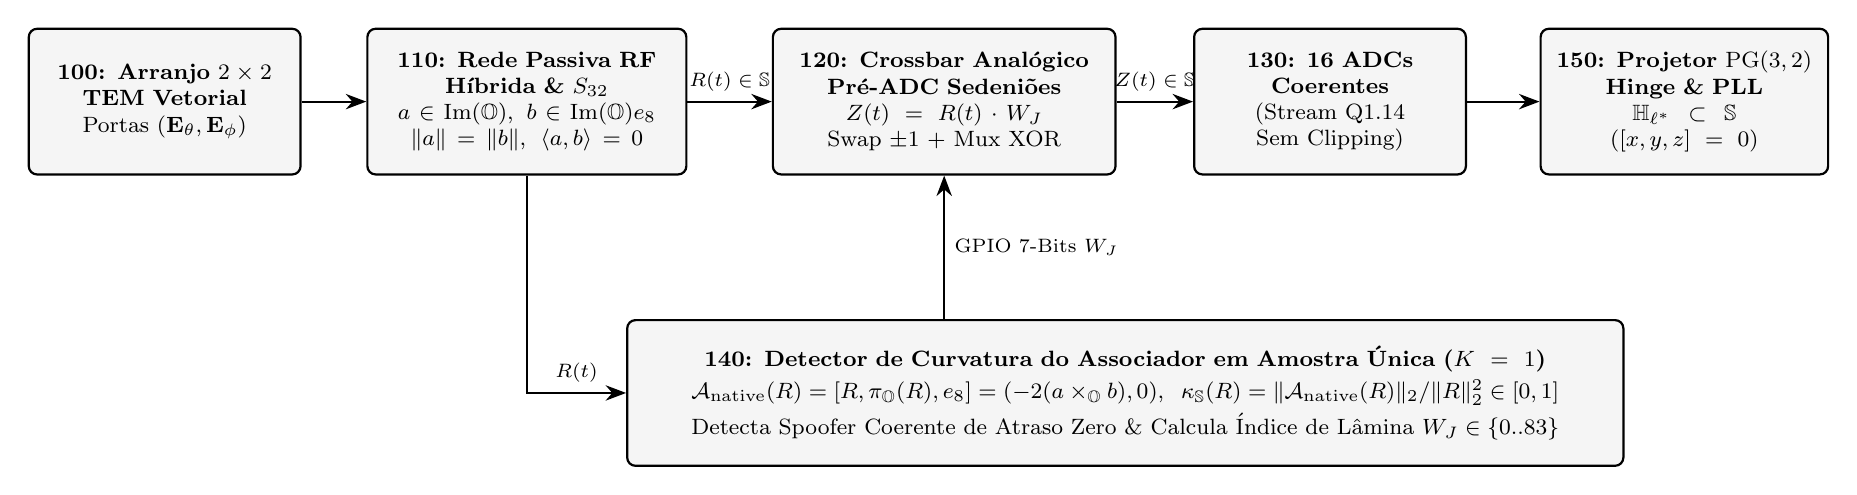
\begin{tikzpicture}[
    font=\footnotesize,
    block/.style={draw, thick, rounded corners=3pt, fill=gray!8, align=center, minimum height=1.85cm, inner sep=5pt},
    arrow/.style={-{Stealth[length=2.6mm]}, thick}
]
    \node[block, text width=3.1cm] (ant) at (0.0, 0) {\textbf{100: Arranjo $2\times 2$}\\\textbf{TEM Vetorial}\\Portas $(\mathbf{E}_\theta, \mathbf{E}_\phi)$};
    \node[block, text width=3.7cm] (hyb) at (4.6, 0) {\textbf{110: Rede Passiva RF}\\\textbf{H\'ibrida \& $S_{32}$}\\$a \in \mathrm{Im}(\mathbb{O}),\; b \in \mathrm{Im}(\mathbb{O})e_8$\\$\|a\|=\|b\|,\; \langle a,b\rangle=0$};
    \node[block, text width=4.0cm] (xbar) at (9.9, 0) {\textbf{120: Crossbar Anal\'ogico}\\\textbf{Pr\'e-ADC Sedeni\~oes}\\$Z(t) = R(t) \cdot W_J$\\Swap $\pm 1$ + Mux XOR};
    \node[block, text width=3.1cm] (adc) at (14.8, 0) {\textbf{130: 16 ADCs}\\\textbf{Coerentes}\\(Stream Q1.14\\Sem Clipping)};
    \node[block, text width=3.3cm] (pll) at (19.3, 0) {\textbf{150: Projetor $\mathrm{PG}(3,2)$}\\\textbf{Hinge \& PLL}\\$\mathbb{H}_{\ell^*} \subset \mathbb{S}$\\($[x,y,z]=0$)};

    \node[block, text width=12.3cm, minimum height=1.85cm] (assoc) at (12.2, -3.7) {\textbf{140: Detector de Curvatura do Associador em Amostra \'Unica ($K=1$)}\\[2pt]
    \mbox{$\mathcal{A}_{\mathrm{native}}(R) = [R, \pi_{\mathbb{O}}(R), e_8] = (-2(a\times_{\mathbb{O}} b), 0), \;\; \kappa_{\mathbb{S}}(R) = \|\mathcal{A}_{\mathrm{native}}(R)\|_2 / \|R\|_2^2 \in [0,1]$}\\[2pt]
    \mbox{Detecta Spoofer Coerente de Atraso Zero \& Calcula \'Indice de L\^amina $W_J \in \{0..83\}$}};

    \draw[arrow] (ant) -- (hyb);
    \draw[arrow] (hyb) -- node[above, font=\scriptsize] {$R(t) \in \mathbb{S}$} (xbar);
    \draw[arrow] (xbar) -- node[above, font=\scriptsize] {$Z(t) \in \mathbb{S}$} (adc);
    \draw[arrow] (adc) -- (pll);
    \draw[arrow] (hyb.south) |- node[pos=0.75, above, font=\scriptsize] {$R(t)$} (assoc.west);
    \draw[arrow] (assoc.north -| xbar.south) -- node[right, font=\scriptsize] {GPIO 7-Bits $W_J$} (xbar.south);
\end{tikzpicture}%
}
\caption{\textbf{FIG.\ 1} --- Arquitetura do Receptor de Processamento Nativo em Sedeni\~oes 16D.}
\end{figure}

\begin{figure}[h!]
\centering
\resizebox{\textwidth}{!}{%
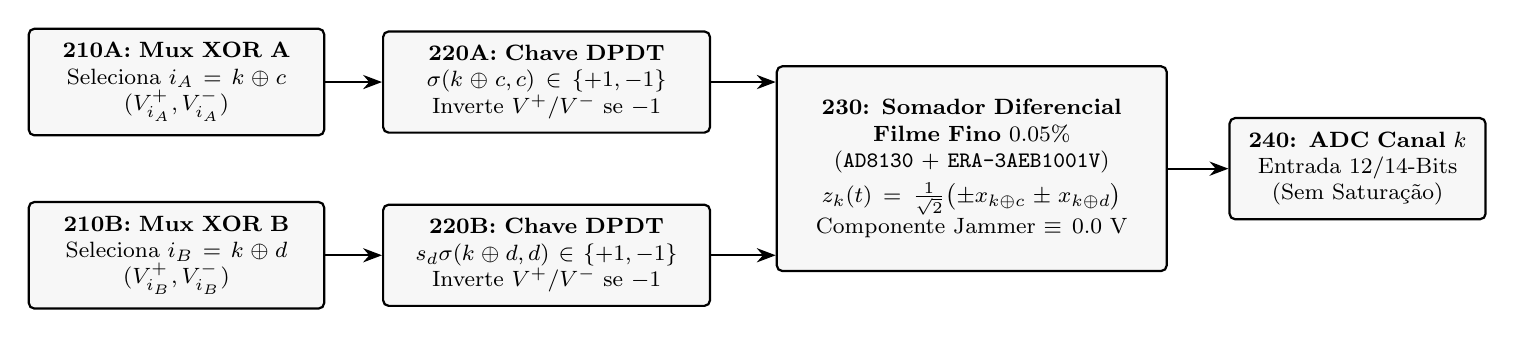
\begin{tikzpicture}[
    font=\footnotesize,
    block/.style={draw, thick, rounded corners=2pt, fill=gray!6, align=center, minimum height=1.15cm, inner sep=5pt},
    arrow/.style={-{Stealth[length=2.4mm]}, thick}
]
    \node[block, text width=3.4cm] (inA) at (0, 1.1) {\textbf{210A: Mux XOR A}\\Seleciona $i_A = k \oplus c$\\$(V_{i_A}^+, V_{i_A}^-)$};
    \node[block, text width=3.4cm] (inB) at (0, -1.1) {\textbf{210B: Mux XOR B}\\Seleciona $i_B = k \oplus d$\\$(V_{i_B}^+, V_{i_B}^-)$};

    \node[block, text width=3.8cm] (polA) at (4.7, 1.1) {\textbf{220A: Chave DPDT}\\$\sigma(k\oplus c, c) \in \{+1,-1\}$\\Inverte $V^+/V^-$ se $-1$};
    \node[block, text width=3.8cm] (polB) at (4.7, -1.1) {\textbf{220B: Chave DPDT}\\$s_d \sigma(k\oplus d, d) \in \{+1,-1\}$\\Inverte $V^+/V^-$ se $-1$};

    \node[block, text width=4.6cm, minimum height=2.6cm] (sum) at (10.1, 0) {\textbf{230: Somador Diferencial}\\\textbf{Filme Fino $0.05\%$}\\(\texttt{AD8130} + \texttt{ERA-3AEB1001V})\\[3pt]
    $z_k(t) = \frac{1}{\sqrt{2}}\bigl(\pm x_{k\oplus c} \pm x_{k\oplus d}\bigr)$\\
    Componente Jammer $\equiv 0.0\text{ V}$};

    \node[block, text width=2.9cm] (adc_k) at (15.0, 0) {\textbf{240: ADC Canal $k$}\\Entrada 12/14-Bits\\(Sem Satura\c{c}\~ao)};

    \draw[arrow] (inA) -- (polA);
    \draw[arrow] (inB) -- (polB);
    \draw[arrow] (polA.east) -- (sum.west |- polA.east);
    \draw[arrow] (polB.east) -- (sum.west |- polB.east);
    \draw[arrow] (sum) -- (adc_k);
\end{tikzpicture}%
}
\caption{\textbf{FIG.\ 2} --- Canal $k \in \{0,\dots,15\}$ do Crossbar Anal\'ogico Diferencial Pr\'e-ADC.}
\end{figure}
\end{document}
